\lecture{15}{Минимакс. Альфа-бета отсечение. Теория Шпрага-Гранди.}
\subsection{Алгоритм минимакс.}
\begin{remark}
  Для игры можно построить дерево игры --- граф игры, расположенный по слоям возможных ходов.
\end{remark}

Такое дерево ходов можно обойти с помощью ретроспективного анализа, но часто:
\begin{itemize}
  \item сложно определить исход игры
  \item сложно оценить минимальное число ходов до выигрыша (максимальное число ходов до проигрыша)
\end{itemize}

Поэтому вводят дополнительную функцию оценки вероятности исхода (приблизительного числа ходов до исхода).
\begin{definition}
  \highlight{Эвристика} --- числовая характеристика игры, зависящая только от состояния игры. 
  Равна $+\infty$ для выигрышных, $-\infty$ для проигрышных.
\end{definition}

Примером эвристики для шахмат, например, может послужить разница между суммы весов своих фигур и суммы 
оппонента.

Рассмотрим теперь алгоритм минимакс, который позволяет получить оценку для всей игры с помощью эвристик.

\begin{enumerate}
  \item Просматриваем дерево, начиная с терминальных вершин, находим их эвристику.
  \item Эвристику следующего уровня смотрим по минимуму (максимуму) всех детей для каждой вершины в дереве
    игры. Минимум или максимум выбирает в зависимости от того, чем сейчас ход. Минимум --- ход оппонента 
    (он старается нам навредить) и максимум для нашего хода.
\end{enumerate}

\begin{figure}[H]    
  \centering    
  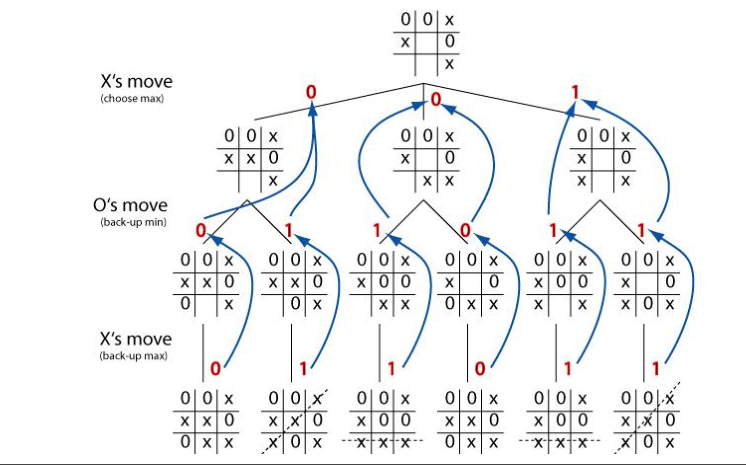
\includegraphics[width=0.8\textwidth]{figures/minmax.png}    
  \caption*{Пример дерева игры для крестиков-ноликов.}        
\end{figure} 

\begin{remark}
  Время работы алгоритма минимакса приблизительно равно коэффициенту ветвления, возведенному в степень числа
  слоёв.
\end{remark}

\subsection{Альфа-бета отсечение.}
Число просмотренных поддеревьев можно уменьшить, если сразу отметать ходы неэффективные для нас.
Пусть мы рассмотрели уже один свой ход $1$ и все возможные ответы соперника и начали рассматривать 
свой второй ход $2$. Как только среди ответов соперника появится такой ход, который ставит нас в ситуацию
хуже, чем самая плохая ситуация, в которую может нас поставить соперник, если мы сходим ходов $1$, то 
можно прекращать перебор возможных ответов соперника на ход $2$ и переходить к рассмотрению следующего нашего
хода.

Значение в узле обозначим за $f(v)$, тогда введём две функции:
\begin{itemize}
  \item $\alpha$ --- текущее максимальное значение оценки узла дял уровня максимизации.
    \[
      \alpha = \max(\alpha, f(v))
    .\] 
    Изначально $\alpha = -\infty$.
  \item $\beta$ --- текущее минимальное значение оценки узла дял уровня минимизации.
    \[
      \beta = \min(\beta, f(v))
    .\] 
    Изначально $\beta = +\infty$.
\end{itemize}

\begin{remark}
  Из определение понятно, что ситуация $\alpha \geq \beta$ эквивалентна описанной выше.
\end{remark}

\begin{figure}[H]    
  \centering    
  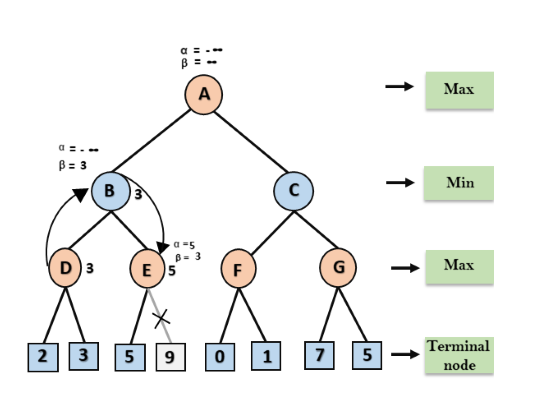
\includegraphics[width=0.6\textwidth]{figures/alpabeta.png}    
  \caption*{Иллюстрация к альфа-бета отсечению.}        
\end{figure} 

\subsection{Теория Шпрага-Гранди.}
\begin{remark}
  Теория Шпрага-Гранди описывает равноправные игры, т. е. игры, в которых ращрешённые ходы зависят только
  от состояния игры. Игроки полность равноправны. Также предполгается что игра конечна. Иными словами,
  такую игру можно полностью описать ориентированным ациклическим графом.
\end{remark}

\begin{definition}
  \highlight{Игра <<Ним>>} --- игра, при которой два игрока по очереди вытаскивают из какой-то кучки камней
  ненулевое число камней. Проигрывает тот, кто не может сделать ход (все кучки пусты).
\end{definition}

\begin{definition}
  \highlight{Прямая сумма игр $A + B$} --- игра, составленная из двух, при которой игрок в начале хода выбирает
  одну из игр, а потом делает в ней ход (нельзя выбрать игру, которая находится в терминальном состоянии).
\end{definition}

\begin{remark}
  Прямая сумма в случае Нима эквивалентна двум кучкам камней (каждую кучку можно рассматривать как отдельную
  игру).
\end{remark}

\begin{remark}
  Прямая сумма коммутативна и ассоциативна, нейтральным элементом относительно неё является игра в
  терминальной вершине, т. е. $A + A_0 = A$.
\end{remark}

\begin{remark}
  Если $A$ --- игра на ациклическом графе, то $A + A$ --- проигрышная игра.
\end{remark}
\begin{proof}
  Оппоненту достаточно применить симметричную стратегию.
\end{proof}

\begin{definition}
  \highlight{Исход игры} --- функция $v(A) = +1$, если $A$ --- выигрышная, $v(A) = -1$, если $A$ ---
  проигрышная. $v(A) = 0$, если $A$ --- ничейная.
\end{definition}

\begin{definition}
  Две игры $A$ и $B$ \highlight{эквивалентны по Гранди} ($A \sim B$ ), если $\forall$ игры $C$ верно:
  \[
    v(A + C) = v(B + C)
  .\] 
\end{definition}
\begin{remark}
  Это отношение является отношением эквивалентности.
\end{remark}

\begin{remark}
  \[
    (A_1 \sim A_2) \wedge (B_1 \sim B_2) \implies (A_1 + B_1) \sim (A_2 + B_2)
  .\] 
\end{remark}
\begin{proof}
  \[
    v((A_1 + B_1) + C) = v(A_1 + (B_1 + C)) = v(A_2 + (B_1 + C)) = v((A_2 + C) + B_1) = v((A_2 + B_2) + C)  
  .\] 
\end{proof}

\subsection{Эквивалентность проигрышных игр.}
\begin{theorem}[Эквивалентность проигрышных]
  Для любой проигрышной игры $L$ и любой игры $C$ выполнено равенство $v(L + C) = v(C)$.
\end{theorem}
\begin{proof}
  Необходимо рассмотреть три случая --- $C$ выигрышная, проигрышная или ничейная.

  Если $C$ выигрышная или проигрышная, то выигрывающий в $C$ игрок (первый или второй, соответственно)
  играет в $C$ в соответствии со своей выигрышной стратегией, а если противник делает ходы в $L$, то
  отвечает в ней в соответствии с выигрышной стратегией в $L$ для второго игрока.

  Пусть теперь $C$ --- ничейная. Проведем индукцию по числу ходов до проигрыша в $L$.

  База очевидна. Если $L$ проигрышная за $0$ ходов, то $L + C$ --- ничейная (в $L$ нельзя сделать ход
  изначально).

  Пусть теперь $L$ проигрышная, и для всех игр, в которых первый игрок проигрывает быстрее чем в $L$, 
  утверждение доказано. Теперь рассмотрим игру $L + C$. Можно ли в ней выиграть?
  
  Делать в таком случае ход в $L$ бессмысленно, т. к. противник точно сможет на него ответить, и задача 
  будет сведена к той же, но проигрыш в $L$ будет за меньшее число шагов. Ходить в $C$ в выигрышную
  позицию также не имеет смысла, т. к. в таком случае противник получил пару из выигрышной и проигрышной 
  игр, в которой выиграет (по доказанному в самом начале). Значит нужно ходить в ничейную позицию, и 
  $L + C$ --- ничейная.
\end{proof}

\begin{remark}
  Если $A$ и $B$ --- проигрышные игры, то $A \sim B \sim A_0$.
\end{remark}

\begin{remark}
  Для любой игры $A$ на ациклическом графе выполняется $A + A \sim A_0$.
\end{remark}

\begin{remark}
  Существует бесконечно много классов эквивалентности выигрышных игр.
\end{remark}

Обозначим за $A_{i}$ игру Ним с одной кучкой в $i$ камней. Очевидно, что $A_0$ --- проигрышная, а
$A_{i}$ --- выигрышная (можно подло взять все камни за раз).
\begin{lemma}
  Игра $A_{i}$ не эквивалентна $A_{j}$ для любых $i \neq j$.
\end{lemma}
\begin{proof}
  Пусть $i < j$. Возьмём в качестве $C$ игру $A_{i}$. Тогда игра $A_{i} + A_{i}$ проигрышная
  (можно использовать симметричную стратегию. С другой стороны, игра $A_{j} + A_{i}$ --- выигрышная.
  Достаточно взять из кучки с $j$ камнями $j - i$ камней, тогда игра сведется к предыдущему случаю.
\end{proof}

\subsection{Теория Шпрага-Гранди для игр на ациклических графах.}
\begin{lemma}{(Об эквивалентности ниму)}
  \[
  A \sim A_{i} \iff A + A_{i} \sim A_0
  .\] 
\end{lemma}
\begin{proof}
  $\implies$
  \[
  A \sim A_{i} \implies A + A_{i} \sim A_{i} + A_{i} \sim A_0
  .\] 
  $\impliedby$
  \[
    A + A_{i} \sim A_0 \implies A \sim A + A_0 \sim A + (A_{i} + A_{i}) \sim (A + A_{i}) + A_{i} \sim 
    A_0 + A_{i} \sim A_{i}
  .\] 
\end{proof}

\begin{theorem}[Шпраг, Гранди]
  Если $A$ --- игра на ациклическом графе, то $\exists i \colon A \sim A_{i}, i = g(A)$. Если из игры
  $A$ существуют ходы в игры $A_1, A_2, \ldots, A_{n}$, то
  \[
    g(A) = mex(g(A_1), g(A_2), \ldots, g(A_{n}))
  ,\] где функция $mex$ от множества чисел возвращает наименьшее неотрицательное числа, не
  встречающееся в этом множестве.
\end{theorem}
\begin{proof}
  Доказательство будем вести по индукции по макимальному пути в графе игры $A$ от начальной вершины
  до терминальной. Если эта длина равна $0$, то начальная вершина $A$ является терминальной, значит
  является проигрышной и эквивалентна $A_0$.

  Пусть для всех игр с длиной максимального пути меньше, чем в $A$, утверждение доказано. Пусть из игры
  $A$ существуют ходы в игры $A_1, A_2, \ldots, A_{n}$. Максимальная длина пути из начальной вершины 
  до терминальной в каждой из этих игр меньше чем в игре $A$, значит по предположению индукции каждая из
  них экзвивалентна игре ним. Выберем $i = mex(g(A_1), g(A_2), \ldots, g(A_{n}))$.

  По предыдущей лемме $A \sim A_{i} \sim A + A_{i} \sim A_0$. Т. е. необходимо доказать, что $A + A_{i}$ 
  --- проигрышная.

  Пусть первый игрок сделал первый ход в игре $A$. Теперь второй игрок будет ходить в сумме 
  $A_{j} + A_{i}$ для некоторого $j$. $A_{j} \sim A_{g(A_{j}}$ (это следует из предположения индукции), 
  $i \neq g(A_{j})$ (по определению $i$ ) $\implies$ $A_{j}$ + $A_{i}$ --- выигрышная (достаточно вспомнить
  стратегию игры при двух кучках камней). 

  Значит первый игрок должен сделать свой ход в игре $A_{i}$. Такой ход возможен в случае $i > 0$.
  После этого хода второй игрок должен делать ход в сумме  $A + A_{k}, k < i$. По определению $i$ --- 
  минимальное число, которое не встречается среди $g(A_1), \ldots, g(A_{n})$, то 
  $\exists j \colon g(A_{j}) = k$. Тогда второй игрок может сделать в $A$ ход в игру $A_{j}$, и 
  первый игрок получит игру $A_{j} + A_{k}$, которая является проигрышной, т. к. $A_{j} \sim A_{k}$ (потому 
  что $g(A_{j}) = k$).

  Значит $A + A_{i}$ проигрышная, значит $A \sim A_{i}$, что и требовалось доказать.
\end{proof} 

\begin{theorem}[Число Гранди суммы игр]
  \[
  A_{i} + A_{j} \sim A_{i \wedge j}
  .\]  
\end{theorem}
\begin{proof}
  Докажем по индукции по сумме $i + j$.

  База: $i + j = 0 \implies (i = 0) \wedge (j = 0) \implies A_{i} + A_{j} = A_0 + A_0 \sim A_0 = A_{i \wedge j}$
  Переход: учитывая предыдущую теорему, для доказательства достаточно показать, что
  \[
    i \wedge j = mex F(i, j)
  ,\] 
  где $F(i, j)$ --- множество чисел Гранди всех игр, в которые возможен ход их игры $A_{i} + A_{j}$:
  \[
    F(i, j) = \left\{ i \wedge 0, i \wedge 1, \ldots, i \wedge (j-1), 0 \wedge j, 1 \wedge j, \ldots, (i - 1) \wedge j \right\} 
  .\] 
  Очевидно, что $i \wedge j$ не лежит в $F(i, j)$. Осталось показать, что все меньшие числа есть в этом 
  множестве.

  Рассмотрим произвольное число $r < i \wedge j$. Пусть $t$ --- номер самого старшего разряда, в котором
  $r$ отличается от $i \wedge j$. Ясно, что $r$ имеет в этом разряде ноль, а $i \wedge j$ --- единицу 
  (т. к. $r < i \wedge j$). Значит $t$-e разряды $i$ и $j$ различны, пусть, без ограничения общности, 
  $t$-й разряд числа $i$ равен единице. 

  Тогда построим число $i'$ таким образом: разряды старше $t$-го в $i'$ сделаем равным соответствующим
  разрядам $i$, $t$-й разряд обнулим, а более младшие выберем так, чтобы выполнялось равенство 
  $i' \wedge j = r$ (мы можем это сделать, потому что меняем в  $i$ только $t$-й бит и младше него).
  
  По построению $i' < i$ (мы обнулили  $t$-й бит), значит по построению  $F(i, j)$ число  $i' \wedge j = r$
  встречается в  $F(i, j)$.

  Значит  $i \wedge j$ является минимальным числом, которое не встречается в множестве $F(i, j)$, а значит
   $A_{i} + A_{j} \sim A_{i \wedge j}$, что и требовалось доказать.
\end{proof}













